% cspell:disable
\documentclass[a4paper,11pt]{article}
% import packages
	\usepackage{amsmath}
	% for source code
	\usepackage[usenames, dvipsnames]{color}
	\usepackage{listings}
	\usepackage{graphicx}

% import babel support for greek
	\usepackage[utf8]{inputenc}
	\usepackage[greek,english]{babel}
	\newcommand{\en}{\selectlanguage{english}}
	\newcommand{\gr}{\selectlanguage{greek}}

% define python style
\lstdefinestyle{Python}{
 language        = Python,
 basicstyle      = \scriptsize\ttfamily,
 keywordstyle    = \bfseries\color{RoyalBlue},
           identifierstyle=\color{RawSienna},
 stringstyle     = \color{Gray},
 commentstyle    = \color{ForestGreen}\ttfamily,
           morecomment =[s]{"""}{"""},
}

% change the abstract name
\addto{\captionsenglish}{\renewcommand{\abstractname}{Rubric Points}} 
%define Q and A template
	\newcounter{question}
	\setcounter{question}{0}
	\newcommand\Que[1]{%
	   \leavevmode\par
	   \stepcounter{question}
	   \noindent
	   Rubric Point \thequestion :  {\bf #1}\par}	
	\newcommand\Ans[2][]{%
    \leavevmode\par\noindent
   {\leftskip37pt
    A --- \textbf{#1}#2\par}}

% define the title
\author{Kostas Oreopoulos}
\title{Project: Kinematics pick \& place}
\date{}
\begin{document}
\lstset{
    frame       = single,
    numbers     = left,
    showspaces  = false,
    showstringspaces    = false,
    captionpos  = t,
    caption     = \lstname,
    style = Python,
    escapechar=@,
}
% generates title
\maketitle
% insert abstract
\begin{abstract}
	Here I will consider the rubric points individually and describe how I addressed each point in my implementation.
\end{abstract}

% Q1
\Que{Provide a Writeup / README that includes all the rubric points and how you addressed each one. You can submit your writeup as markdown or pdf.}
\Ans{You are reading it}

\section{Kinematic Analysis}
% Q2
\Que{Run the forward kinematics demo and evaluate the kr210.urdf.xacro file to perform kinematic analysis of Kuka KR210 robot and derive its DH parameters.}
\Ans{Based on the kr210.urdf.xacro file, the forward kinematics demo and the joint diagram of Kuka KR210 as presented in lessons and following the same numbing of joints I derived the Denavit--Hartenberg parameters as show in table~\ref{table:dh parameters}.}
\begin{table}[!h]
	\caption{Denavit -- Hartenberg parameters for the Kuka KR210 arm robot}
	\label{table:dh parameters}
	\begin{center}
		\begin{tabular}{ | c | c | c | c | c | }
			\hline
			{\bf i} & $\boldsymbol \alpha_{i-1}$ & $\mathbf a_{i-1}$ & $\mathbf d_{i}$ & $\boldsymbol \theta_{i}$ \\ [0.5ex] 
			\hline
			\rule{0pt}{1.2em}1 & $0$ & $0$ & $0.75$ & $\theta_{1}$ \\ 
			2 & $-\pi/2$ & $0.35$ & $0$ & $\theta_{2}$ \\
			3 & $0$ & $1.25$ & $0$ & $\theta_{3}$ \\
			4 & $-\pi/2$ & $-0.054$ & $1.5$ & $\theta_{4}$ \\
			5 & $-\pi/2$ & $0$ & $0$ & $\theta_{5}$ \\
			6 & $-\pi/2$ & $0$ & $0$ & $\theta_{6}$ \\
			7 & $-\pi/2$ & $0$ & $0.303$ & $0$ \\
			\hline
		\end{tabular}
	\end{center}
\end{table}
% Q3
\Que{ Using the DH parameter table you derived earlier, create individual transformation matrices about each joint. In addition, also generate a generalized homogeneous transform between base\_link and gripper\_link using only end-effector(gripper) pose.}
\Ans{To derive the individual transformation matrices about each joint I created a small python function that takes the DH parameters for each transformation and generates the appropriate matrix. I used the code in listing~\ref{code:DH parameters}.

Also to account for the different orientation of the frames in DH parameters and the frame as defined in the URDF file for the end effector I calculated a correction matrix that is simply an 180 degrees rotation on the z--axis, followed by one around y axis by -90 degrees. The code is available in listing~\ref{code:correction matrix}}
 
\begin{lstlisting}[language=Python, caption={Transformation Matrix based on DH parameters}, label={code:DH parameters}]
def dh_transformation(theta_x, d_dz, theta_z, d_dx):
    """
    Calculate the transformation matrix based on the
    Denavit - Hartenberg parameters
    :param  theta_x: @$\alpha$@ dh parameter. rotation (twist) around x axis
    :param  theta_z:  @$\theta$@ dh parameter. rotation around z axis
    :param  d_dz: a dh parameter. length of x_i-1 (common normal)
                  between z_i-1 and z_i
    :param  d_dx: d dh parameter. displacement of x axis
                  measured along z axis
    :return:
    """
    return Matrix([[cos(theta_z), -sin(theta_z), 0, d_dz],
                   [sin(theta_z) * cos(theta_x), 
                    cos(theta_z) * cos(theta_x),
                    -sin(theta_x),
                    -sin(theta_x) * d_dx],
                   [sin(theta_z) * sin(theta_x),
                    cos(theta_z) * sin(theta_x),
                    cos(theta_x),
                    cos(theta_x) * d_dx],
                   [0, 0, 0, 1]])

\end{lstlisting} 


\begin{minipage}{\linewidth}
\begin{lstlisting}[language=Python, caption={Correction Matrix}, label={code:correction matrix}]
def correction_matrix():
"""
A matrix to transform the end effector frame such as to align
with the URDF specs
"""
r_z = Matrix([[cos(pi), -sin(pi), 0, 0],
[sin(pi), cos(pi), 0, 0],
[0, 0, 1, 0],
[0, 0, 0, 1]])
r_y = Matrix([[cos(-pi / 2), 0, sin(-pi / 2), 0],
[0, 1, 0, 0],
[-sin(-pi / 2), 0, cos(-pi / 2), 0],
[0, 0, 0, 1]])
return simplify(r_z * r_y)
\end{lstlisting}
\end{minipage}

% Q4
\Que{ Decouple Inverse Kinematics problem into Inverse Position Kinematics and inverse Orientation Kinematics; doing so derive the equations to calculate all individual joint angles.}
\Ans{By design the end effector of the robot arm is rigidly attached to the robots wrist center, extending by 0.303m. That means that the orientation of the end effector is the same as the one of the wrist center, which means that $R^6_7 = Identity$ and $R^3_7 = R^3_6$. \\
We can also calculate the position of the wrist center by the equation $\vec{WC}= \vec{EE} - R^0_6*(0.303, 0 , 0)^T$ , where all quantities are expressed in the 0th frame.

Our next step is to calculate $R^0_3$, which will by the equation $R^3_6 = (R^0_3)^{-1}*R^0_6 = (R^0_3)^T*R^0_6$, will also give us $R^3_6$. From that step and using what we learned in Lesson 2.18 we can extract the Euler angles of the wrist center, concluding our Inverse Kinematics task.

To find the first three angles of the IK problem we will use figure \ref{fig:angles}. In it, Point A is joint 2, point B is joint 3 and point C is joint 4. The following equations hold
\begin{equation}
\gamma = pi/2 - theta_3 + \text{initial angle}
\label{eq:initialgamma}
\end{equation}
\begin{equation}
\text{initial angle} = \arctan(-0.054, 1.5)
\end{equation}
\begin{equation}
\cos(\gamma) = \frac{\left(|\vec{AC}|^2 - |\vec{AB}|^2 - |\vec{BC}|^2\right)}{-2|\vec{AB}||\vec{BC}|}
\end{equation}
\begin{equation}
\gamma = \arctan(\sqrt{1-cos^2(\gamma)}, cos(\gamma))
\label{eq:gamma}
\end{equation}
\\
From \ref{eq:initialgamma} and \ref{eq:gamma} we get $theta_3$. Next we find $theta_2$ which is $\alpha$ in the figure. We also note that angles $E\hat{A}H$ and $E\hat{C}B$ are equal because they have their corresponding sides perpendicular. By that fact the following equations hold:

\begin{equation}
\alpha = theta_3 = \delta + \epsilon
\label{eq:initialtheta3}
\end{equation}
\begin{equation}
\epsilon =  \arctan(HB,HC) = \arctan(AB - \overbrace{\cos(\gamma)BC}^{HA} ,\sin(\gamma)BC)
\end{equation}
\begin{equation}
\delta =  \arctan(AD,DC)
\end{equation}
}

We conclude by calculating $theta_1$ which is the easiest of all, since $ theta_3 =\arctan(\text{wrist\_center}_y,\text{wrist\_center}_x)$.
\begin{figure}[hbt!]
	\caption{Joint - Angle configuration}
	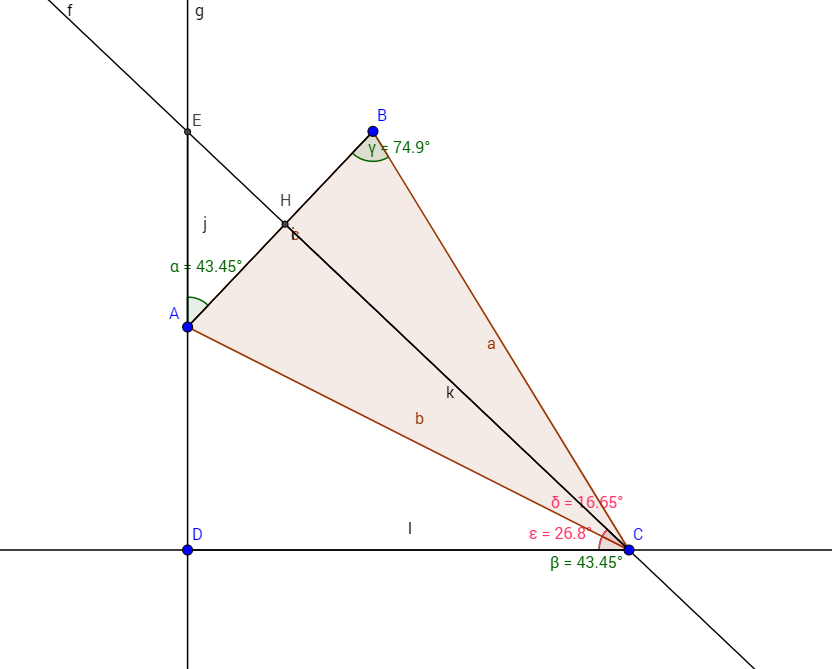
\includegraphics[scale=0.8]{geogebra_joints.png}
	\label{fig:angles}
\end{figure}

\section{Project Implementation}
% Q4
\Que{ Fill in the IK\_server.py file with properly commented python code for calculating Inverse Kinematics based on previously performed Kinematic Analysis. Your code must guide the robot to successfully complete 8/10 pick and place cycles. Briefly discuss the code you implemented and your results.}
\Ans{The implementation of the python code is a straightforward application of the above formulas. The code does the following:
\begin{itemize}
	\item Sets up all transformation matrices.
	\item Calculates a correction matrix for the misalignment of EE frame and URDF file frame
	\item Calculates the t\_FK transform which is the final transform between frame 0 an EE frame.
	\item Uses all formulas discussed above, in the inverse\_kinematics function and calculates angles theta\_1 to theta\_6 
	\item All the above are done symbolically and once when the program begins.
	\item Once a pose is received, function {\em calculateFromPose} applies the values to the closed form formulas and returns the requests angles
	\item As a last step, forward kinematics are applied to the calculated angles and the point predicted is compared with the ground truth (pose data) and an error is calculated per pose and stored in an array. At the end of a batch of poses, the average error is calculated and reported.
	\item The code performs 8 or 9 out of 10 tries and when it misses, it is because the arm throws the cylinder of the self (something that probably has more to do with path planning than calculation of the inverse kinematics)
	
\end{itemize}
}
\end{document}